\section{Astronomy Terms}
\subsection{The Celestial Sphere}
The celestial sphere is a fundamental concept in astronomy.
It is an imaginary sphere with an arbitrary radius that is centered on Earth, and it allows us to represent the positions of celestial objects in a convenient and intuitive way.
Any astronomical observation can be thought of as a 2D projection onto the celestial sphere, which is a tool that astronomers use to specify the position of a target without using its distance.
Instead, the position is described in terms of two-dimensional coordinates on the sphere.
While the celestial sphere is a universal concept, the coordinate system used to specify the location of a target can vary from telescope to telescope.




\subsection{Altitude-Azimuth Coordinate System}
Figure \ref{fig:altaz_coords} depicts the coordinate system used at APEX, which is an altitude-azimuth system.
In this system, coordinates are specified using an azimuth and an altitude (or elevation) angle.
Azimuth is the angle around the axis perpendicular to the horizontal plane, with zero degrees corresponding to due north.
At APEX, the convention is to increase the azimuth angle in a clockwise direction.
The interval for azimuth angles is $[-270^\circ,270^\circ]$ due to APEX's ability to rotate one and a half times around its own axis in the horizontal plane.
Elevation, on the other hand, is the angle perpendicular to the horizontal plane, with zero degrees corresponding to the telescope pointing at the horizon, and $90\degr$ to the telescope pointing at zenith, which is directly above it.
Throughout this thesis, we will use the term elevation instead of altitude to describe this coordinate.\\

Another angle term used in this thesis is the horizontal angle.
We will use the term azimuth when referring to the telescope pointing, while the term horizontal angle will be used for the pointing offset.
The azimuth angle is the angle projected on the horizontal plane, while the horizontal angle is the angle measured on the celestial sphere and is dependent on elevation.
It is important to be aware of this distinction when measuring offsets, and applying it corrections to the pointing model.

For example, suppose we are pointing at a source at $Az=El=60\degr$ and observe that the source is actually $1\degr$ to the right.
In this case, the horizontal offset is $1\degr$, while the azimuth offset is $1\degr/\cos{El}=2\degr$.
Therefore, the azimuth angle must be increased by twice the horizontal offset due to the influence of elevation.

\begin{figure}[H]
    \centering
    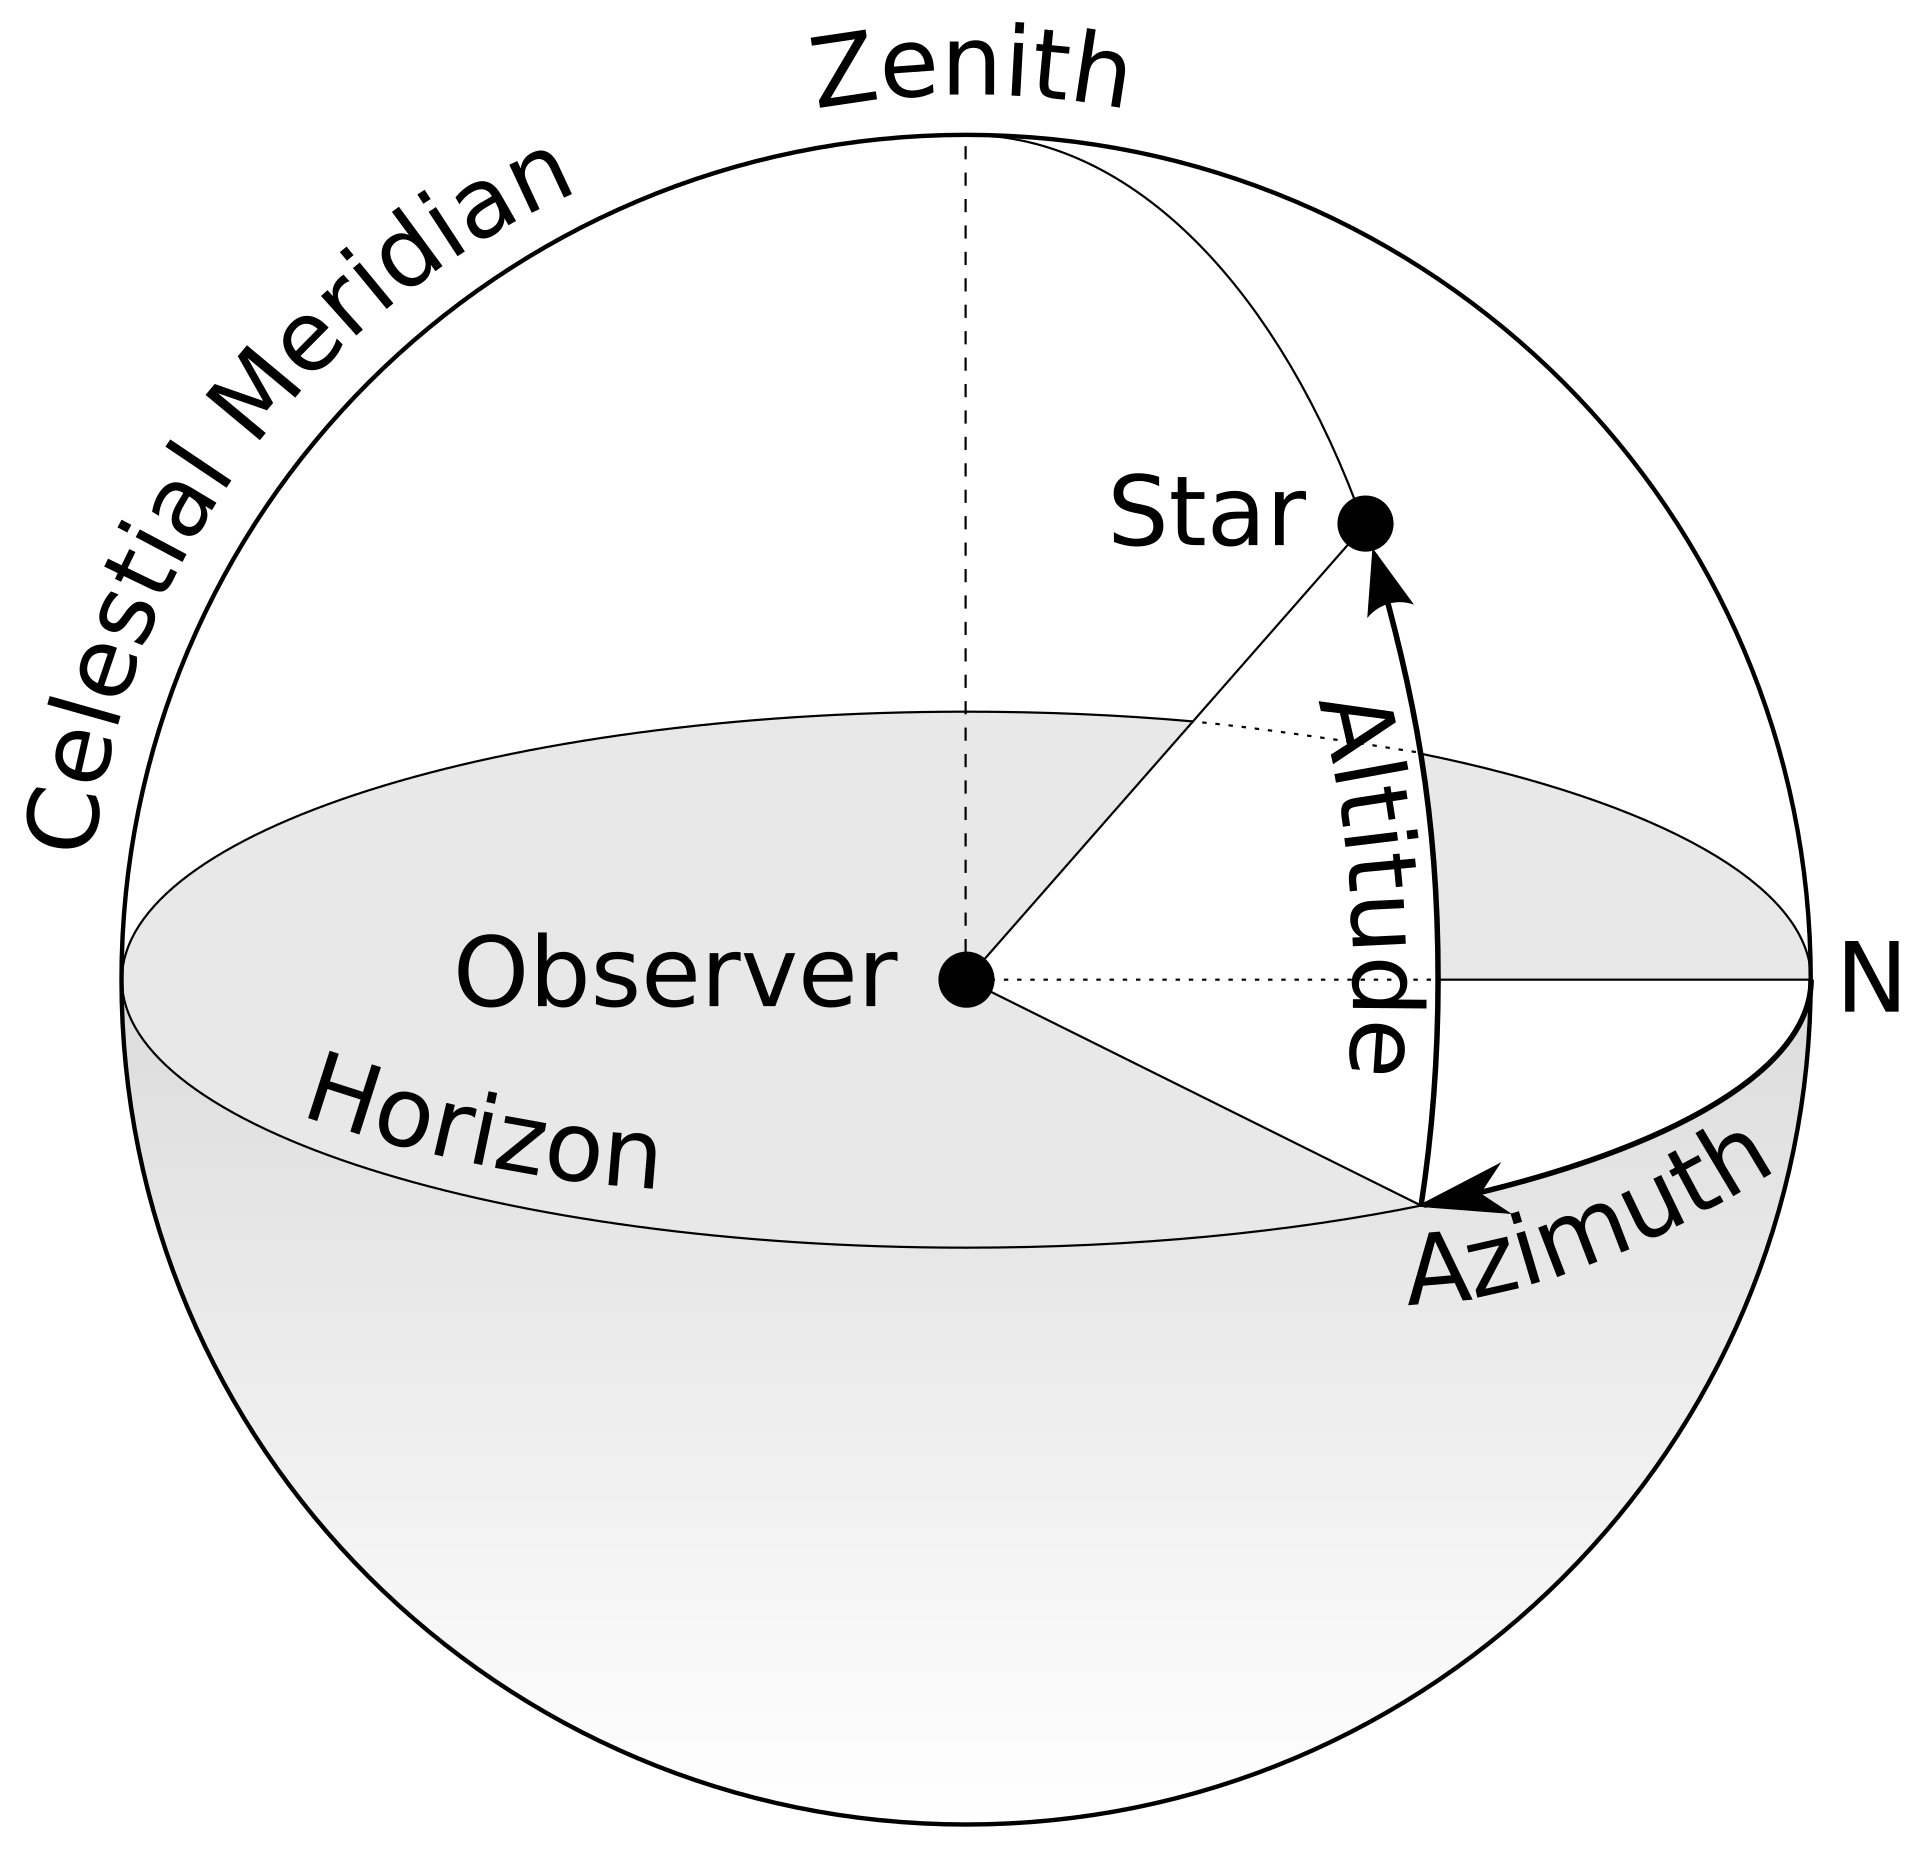
\includegraphics[width=0.98\textwidth]{Astronomy/Azimuth-Altitude_schematic.png}
    \caption{The altitude-azimuth coordinate system used at APEX. Source \cite{altaz_schematic}}
    \label{fig:altaz_coords}
\end{figure}




\section{Radio/(sub)-mm telescope basics}





\begin{figure}[H]
    \centering
    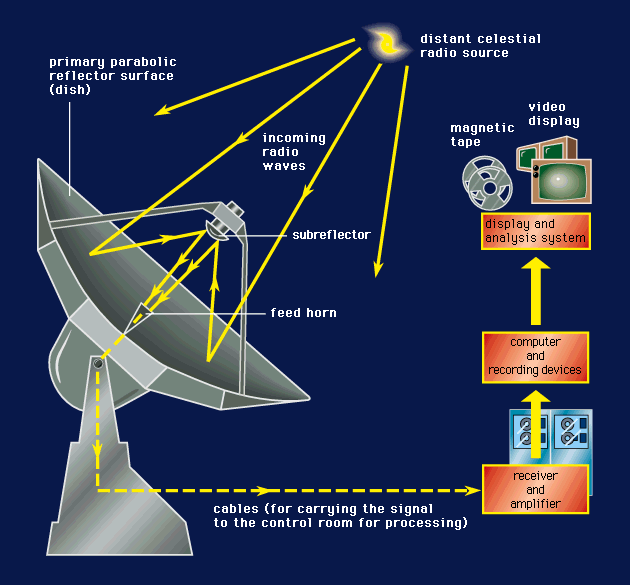
\includegraphics[width=0.98\textwidth]{Astronomy/radio_telescope.png}
    \caption{The main parts of a radio telescope.}
    \label{fig:radio_telescope}
\end{figure}


\section{Problem description}
\textcolor{red}{This section have to be fixed completely}
A telescope makes high precision observations of objects located very far away from earth.
Because of this distance, small changes such as deformation of mirrors due to temperature might impact the precision drastically.\cc{Claudia Cicone: Here you could explain that astronomical objects are observed as they were "projected" in 2D angular coordinates on the sky, and you could talk about astronomical coordinates (see Lecture 5 notes of my course AST2210 for some explanation and references)
}
Over time, these deformations have been observed and analyzed, and in order to counter this, a pointing model is made.
\cc{Claudia Cicone: The need for a pointing model is relevant mainly to sub-mm telescopes that cannot take real-time images of what they are observing, and so the precision of the pointing direction must be known accurately before starting the observations.}
The pointing model uses measurements from various instruments, and is fitted to the observed offsets.
The model is used for about a month, or until it start performing poorly.
The variation in measurements are still too big using only this model, so pointing scans have to be made regularly to correct even more.
A pointing scan is an observation of an object with known location.
When doing this, the offset on this observation is then added on top of the pointing model.
These corrections to azimuth and elevations are used for a couple of hours, until a new pointing scan is made.
\cc{Claudia Cicone: Need to define azimuth and elevation first, see other comment above
}
Using this approach, pointing error is reduced to about $4$ arc seconds.\\

The aim of this thesis is to investigate the possibility of using machine learning to increase the performance of the telescope, by improving pointing accuracy.
This can be done in multiple ways.

One possibility is to apply a pointing model on top of the current pointing model using machine learning, such that the average offset is reduced even more.
Another possibility is investigating the use of machine learning models to aid such that a pointing scan doesn't have to be made as often.
This will reduce the workload at the telescope. \\

\section{Pointing model}
Since radio/(sub)-mm telescope observe over extended time, they need a pointing model to obtain sufficiently accurate pointings.
The flux of the brightest radio sources are also weaker than the atmospheric emission, which means that they are invisible in real time.
Therefore, the astronomers need to know that the pointing is accurate before making observations.
The pointing model at APEX consists of two parts, one analytical model, and additional pointing corrections performed at regular intervals based on recent observed pointing offsets.
The resulting pointing can be explained by these equations
\begin{align}
    Az &= Az_\text{input} + \Delta Az_\text{analytical model} + \Delta Az_\text{correction} \\ 
    El &= El_\text{input} + \Delta El_\text{analytical model} + \Delta El_\text{correction}
\end{align}
Where the first term is the input coordinates, the second is the adjustment made according to the analytical model,
and the last term is the adjustments made according to recent observed pointing offsets.

In the following section, I introduce and explain the adjustments from the analytical model and pointing offsets. 


\subsection{Analytical model}
\textcolor{red}{How good is this model, and how accurate after pointing corrections?}
There are a lot of different factors that affect the pointing, 
and some of them can be modelled with an analytical model. Some of the terms are purely geometrical, based on imperfect mounting of telescope components,
and others are empirical. The following terms are the ones used in the analytical pointing model at APEX,
and the description of them are taken directly from the tpoint software manual \cite{tpoint_manual}.
All the terms are dependant on either the azimuth $Az$ or elevation $El$, except for a couple that are just constants. 
The sum of all the terms is the adjustment adjustment made by the model.
All the constants are determined by a linear fit based on observed offsets from a pointing campaign.


\subsubsection{Harmonic terms}
There are multiple harmonic terms in the analytial model, some geometrical and some empirical.
The empirical terms have been found to improve the model through trial and error.
The following terms are the empirical terms for azimuth
\begin{align}
    \Delta Az =&  c_1 \cdot \sin{Az} + c_2 \cdot \frac{\cos{2Az}}{\cos{El}} + c_3 \cdot \cos{3Az} + c_4 \cdot \sin{2Az} \\
    &+ c_5 \cdot \cos{2Az} + c_6 \cdot \frac{\cos{Az}}{\cos{El}} + c_7 \cdot \frac{\cos{5Az}}{\cos{El}},
\end{align}
and the terms for elevation are

\begin{align}
    \Delta El =&  c_1 \cdot \sin{El} + c_2 \cdot \cos{El}+ c_3 \cdot \cos{2Az} + c_4 \cdot \sin{2Az} \\
    &+ c_5 \cdot \cos{3Az} + c_6 \cdot \sin{3Az} + c_7 \cdot \sin{4Az} + c_8 \cdot \sin{5Az}  
\end{align}


In the tpoint software, harmonic terms are denoted on the format $Hrfci$. The list below explain the different terms.
\begin{itemize}
    \item $H$: Stands for harmonics
    \item $r$: The resulting variable, either $Az$ or $El$, denoting azimuth and elevation respectively.
    The resulting variable can also be $S$, which means result is horizontal, or azimuth scaled by a factor $1/\cos{El}$.
    \item $f$: The harmonic function, either $S$ or $C$ denoting \textit{sine} and \textit{cosine}.
    \item $c$: The variable that the funciton $f$ is dependent on, either $Az$ or $El$.
    \item $i$: Integer value in the range $0$-$9$, denoting the frequency of the harmonic.
\end{itemize}

For example will $\Delta Az = \text{HACA3}\cos{3Az}$ be denoted as HACA3 in the software.

\subsubsection{Az/El non-perpendicularity (NPAE)}
In an altazimuth mount, if the azimuth axis and elevation axis are not exactly at
right angles, horizontal shifts proportional to $\sin{El}$ occur. This effect is zero when pointing at the horizon, and increases with elevation propotional to $1/\cos{El}$

\begin{equation}
    \Delta Az \simeq - \text{NPAE } \frac{\sin{El}}{\cos{El}}= - \text{NPAE } \tan{El},
\end{equation}
where NPAE is the horizontal displacement when poining at Zenith.

\subsubsection{Horizontal displacement of Nasmyth rotator}
In a Nasmyth altazimuth mount, a horizontal displacement between the elevation axis of the mount and the rotation axis of the Nasmyth instrument-rotator produces
and image shift on the sky with a horizontal component
\begin{equation}
    \Delta Az \simeq - \text{NRX},
\end{equation}
and an elevation component
\begin{equation}
    \Delta El \simeq - \text{NRX} \sin{El},
\end{equation}
where NRX is the horizontal displacement.

\subsubsection{Left-right collimation error}
In an altazimuth mount, the collimination error is the non-perpendicularity between the nominated pointing direction and the elevation axis.
It produces a horizontal image shift given by
\begin{equation}
    \Delta Az \simeq -\text{CA} \sec{El}
\end{equation}


\subsubsection{Azimuth and elevation index error}
Index errors are the errors when you point at the origo.

The azimuth index error is 
\begin{equation}
    \Delta Az = -\text{IA},
\end{equation}

and elevation index error is
\begin{equation}
    \Delta El = \text{IE}
\end{equation}

\subsubsection{Azimuth axis misalignment} 

In an altazimuth mount,misalignment of the azimuth axis north-south or east-west cause errors.
The errors cause by misalignment in north-south are given by

\begin{equation}
    \Delta Az \simeq - \text{AN} \sin{Az} \cdot \tan{El},
\end{equation}

and

\begin{equation}
    \Delta El \simeq - \text{AN} \cos{Az},
\end{equation}
where AN is the misalignment alignent in north-south direction.
The errors given by misalignment in east-west are given by

\begin{equation}
    \Delta Az \simeq - \text{AW} \cos{Az} \tan{El},
\end{equation}

and

\begin{equation}
    \Delta El \simeq \text{AW} \sin{Az},
\end{equation}
where AW is the misalignment alignent in east-west direction.



\subsection{Pointing corrections} 
The analytical pointing model can only reduce the pointing offsets down to about an average of \textcolor{red}{$x$ arcseconds}.
To reduce the pointing offsets even further, a pointing scan is made by pointing the telescope at a source with known coordinates. 
This operations is called a pointing scan, and by observing the resulting pointing offsets from the known source,
the pointing model can be updated according to the following eqautions
The terms $\Delta Az_\text{correction}$ and $\Delta Az_\text{correction}$ are updated
\begin{align}
    \Delta Az_\text{correction} &= \Delta Az_\text{correction} + \delta_{\text{Az}} \label{eq:ca}\\ 
    \Delta El_\text{correction} &= \Delta El_\text{correction} - \delta_{\text{El}},\label{eq:ie}
\end{align}
where $\delta_{\text{Az}}$ and $\delta_{\text{El}}$ are the recently observed pointing offsets in azimuth and elevation respectively.
These pointing corrections are carried out every couple of hours to make sure the pointing is sufficient during science observations.

In the telescope systems, the correction variables $\Delta Az_\text{correction}$ and $\Delta El_\text{correction}$ are labeled as $ca$ and $ie$ respectively,
and I will therefore refer to them as such in the rest of this thesis.

\section{Research questions and related works}
\begin{itemize}
    \item Reduce poitning offsets with machine learning model
    \item Replace analytical model with machine learning model
    \item reduce the frequency of pointing scans while maintaining pointing accuracy with machine learning model
\end{itemize}

\begin{itemize}
    \item Article about analytical model
    \item ...
\end{itemize}

\section{Database}


\subsection{Optical Observations}
The analytical model relies on observations obtained through an optical receiver.
Optical observations are easier to obtain when there is no other pointing model, as you can observe the source in real time.
To obtain the necessary data, the telescope is pointed at various sources with known locations.
This process yields both input coordinates and actual observed coordinates, and can be done for the different instruments at the telescope.
According to astronomers at the telescope, only the NFLASH230 receiver have reliable and consistent optical observations, as the data obtained using the other receivers
are too noisy due to structural changes at the telescope. Therefore, only optical data from NFLASH230 is used for the analytical underlying poinitng model in this project.

Table \ref{tab:optical} provides an example of the format of this data.
    

\begin{table}[h]
    \centering
    \begin{tabular}{ccccc}
         & \multicolumn{2}{c}{Input} & \multicolumn{2}{c}{Observed} \\ 
        \cline{2-3} \cline{4-5}
        Date & Azimuth & Elevation & Azimuth & Elevation \\ 
        \hline \\
        2022-01-03 14:24:04 & $189.812879$ & $41.0762$ & $190.254779$ & $40.883651$ \\
        2022-01-03 18:59:40 & $50.842145$ & $73.371647$ & $51.269044$ & $73.203243$ \\
        2022-01-03 19:01:49 & $49.555916$ & $73.752182$ & $49.983112$ & $73.583545$ \\
        2022-01-03 19:16:10 & $39.378382$ & $76.076236$ & $39.781084$ & $75.908956$ \\
        2022-01-03 19:18:27 & $113.934309$ & $39.345667$ & $114.391232$ & $39.170168$ \\
        2022-01-22 13:54:31 & $94.04365$ & $18.148405$ & $94.492505$ & $17.981161$ \\
        2022-01-22 14:15:35 & $148.569964$ & $89.044036$ & $147.783271$ & $88.852306$ \\
        2022-01-22 14:18:15 & $215.664924$ & $49.563821$ & $216.104389$ & $49.386438$ \\
    \end{tabular}
    \caption{Extract from data obtained by the optical receiver of NFLASH230. The source is also included in the datafile, but it is not relevant here. \textcolor{red}{I don't know what it means that optical data is for the nflash receiver}}
    \label{tab:optical}
    \end{table}




\subsection{The Monitor Database}
The monitor database plays a critical role in this project, providing valuable sensory data from within and outside of the telescope.
In this section, we will explore the data contained within the monitor database and identify the variables that are most relevant for our purposes.

\paragraph{Azimuth and Elevation}
The database have tables for the input azimuth and elevation, which is the raw coordinates before the main pointing model have adjusted the pointing.
These are labeled COMMANDAZ and COMMANDEL.
In addition to these, it includes the actual azimuth and elevation, which is the result after applying the pointing model, and a correction obtained from a pointing scan.
These are labeled ACTUALAZ and ACTUALEL.

Additionally, the database contains tables for the velocity of the azimuth and elevation, labeled ACTUALVELOCITYAZ and ACTUALVELOCITYEL.

\paragraph{Temperature Measurements}
Temperature is measured by multiple instruments at various locations on the telescope.
The database includes tables labeled as TEMPERATURE, TEMP1 through TEMP6, TEMP26 through TEMP28, and TILT1T.
Figure \ref{fig:corr_temp} shows that many of these measurements are highly correlated.
Specifically, TEMP1 through TEMP6 are all correlated with each other at a coefficient of $\geq 0.98$.
Similarly, TEMP26 through TEMP28 and TEMPERATURE are also highly correlated.

\begin{figure}[H]
    \centering
    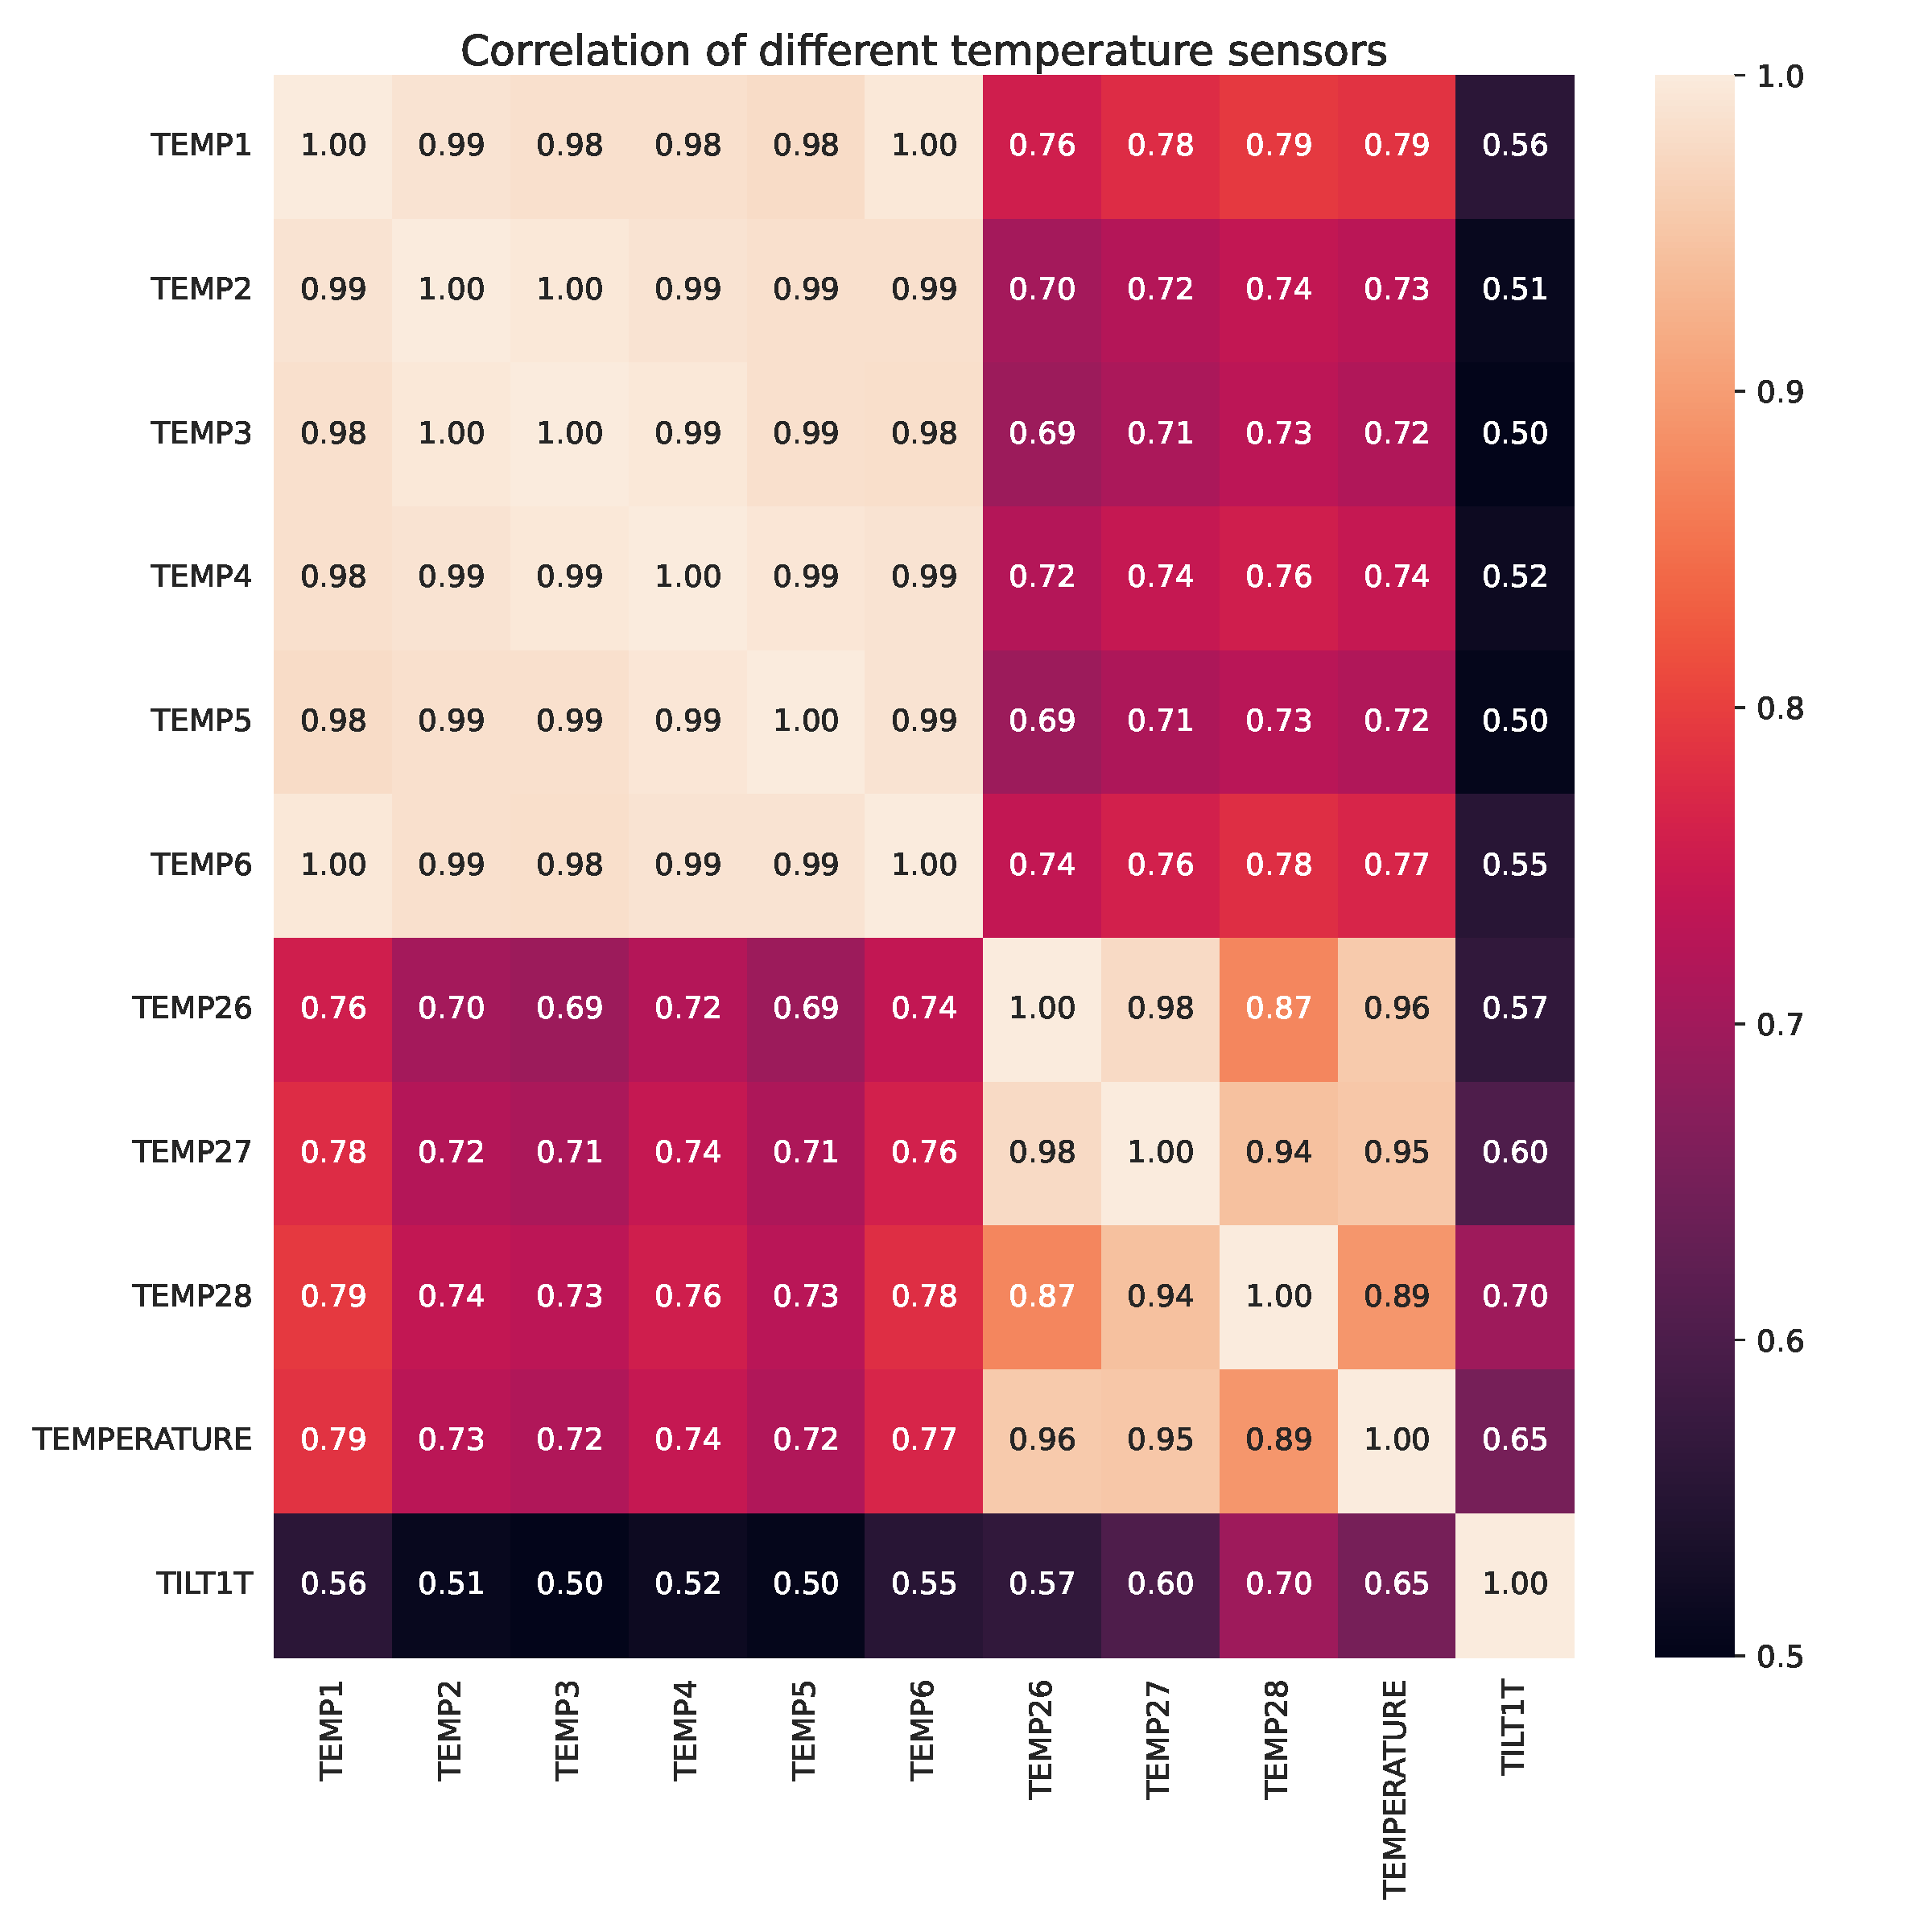
\includegraphics[width=0.98\textwidth]{Correlation/Correlation_temp.pdf}
    \caption{Linear correlation between temperature measures.
    The values are the median of all data points within a pointing scan.}
    \label{fig:corr_temp}
\end{figure}

\paragraph{Hexapod}
The secondary mirror, also known as the subreflector, is supported by a hexapod. 
The hexapod is capable of three-dimensional movement and can also rotate around the azimuth and elevation axes.
There are five measures associated with the hexapod: POSITIONX, POSITIONY, POSITIONZ, ROTATIONX, and ROTATIONY.
These measures are essential for positioning the secondary mirror and ensuring an accurate pointing.

\paragraph{Tiltmeter}
The telescope is equipped with two tiltmeters that measure the tilt or inclination of the telescope with respect to the vertical direction.
One of the tiltmeters is aligned with the telescope pointing direction, while the other is orthogonal to it.
These tiltmeters are labeled TILT1X and TILT1Y, respectively.

\paragraph{Weather data}
The weather station at the telescope provides measurements of various weather parameters, including dew point, humidity, pressure, wind speed, and wind direction.
The instruments take measurements at an interval of $11$ seconds.


\textcolor{red}{Put this in feature engineering section}
\begin{align}
    \Delta \textit{Az}_\textit{wind} = \textit{Az}_\textit{pointing} - \textit{Az}_\textit{wind}
\end{align}

For the turbulence, a simple model is used
\begin{align}
v_\textit{wind} = \sigma_\textit{wind}^2
\end{align}

\paragraph{Disp abs?}

\paragraph{Automatic adjustments}
To ensure accurate and stable pointing of the telescope, there are automatic adjustments made based on readings from various sensors.
These adjustments account for systematic errors that have been previously modeled and are based on measurements from tiltmeters,
temperature sensors installed at different locations, and other relevant sources of data \textcolor{red}{Explain spem and disp here?}.
The automatic adjustments are made in the azimuth and elevation directions and are denoted by variables starting with DAZ or DEL, respectively.
A comprehensive list of these variables can be found in Table \ref{tab:data_frequency}.

\paragraph{Data frequency}
The monitor database provides data with varying frequencies, as shown in Table \ref{tab:data_frequency}, which lists the approximate number of data points per minute.

\begin{table}[H]
    \caption{The frequency in datapoints per minute of different variables in the monitor database.}
    \centering
    \begin{tabular}{lr}
        \toprule
        Table &  Frequency [datapoints/minute] \\
        \midrule
        ACTUALAZ &                    6 \\
        ACTUALEL &                    6 \\
        ACTUALVELOCITYAZ &                    6 \\
        ACTUALVELOCITYEL &                    6 \\
        COMMANDEL &                    6 \\
        COMMANDAZ &                    6 \\
        TILT1X &                   12 \\
        TILT2Y &                   12 \\
        TILT1T &                   12 \\
        TEMPERATURE &                    5 \\
        TEMP1 &                    6 \\
        TEMP2 &                    6 \\
        TEMP3 &                    6 \\
        TEMP4 &                    6 \\
        TEMP5 &                    6 \\
        TEMP6 &                    6 \\
        TEMP26 &                    2 \\
        TEMP27 &                    2 \\
        TEMP28 &                    2 \\
        DAZ\_TEMP &                   12 \\
        DAZ\_TILT &                   12 \\
        DAZ\_TILTTEMP &                   12 \\
        DAZ\_SPEM &                   12 \\
        DAZ\_DISP &                   12 \\
        DAZ\_TOTAL &                   12 \\
        DEL\_TEMP &                   12 \\
        DEL\_TILT &                   12 \\
        DEL\_TILTTEMP &                   12 \\
        DEL\_SPEM &                   12 \\
        DEL\_DISP &                   12 \\
        DEL\_TOTAL &                   12 \\
        POSITIONX &                    6 \\
        POSITIONY &                    6 \\
        POSITIONZ &                    6 \\
        ROTATIONX &                    6 \\
        ROTATIONY &                    6 \\
        DISP\_ABS1 &                   12 \\
        DISP\_ABS3 &                   12 \\
        DISP\_ABS2 &                   12 \\
        DEWPOINT &                    5 \\
        PRESSURE &                    5 \\
        HUMIDITY &                    5 \\
        WINDSPEED &                    5 \\
        WINDDIRECTION &                    5\\
        \bottomrule
    \end{tabular}
    \label{tab:data_frequency}
\end{table}


\begin{figure}[H]
    \centering
    \begin{subfigure}[t]{0.49\textwidth}
        \centering
        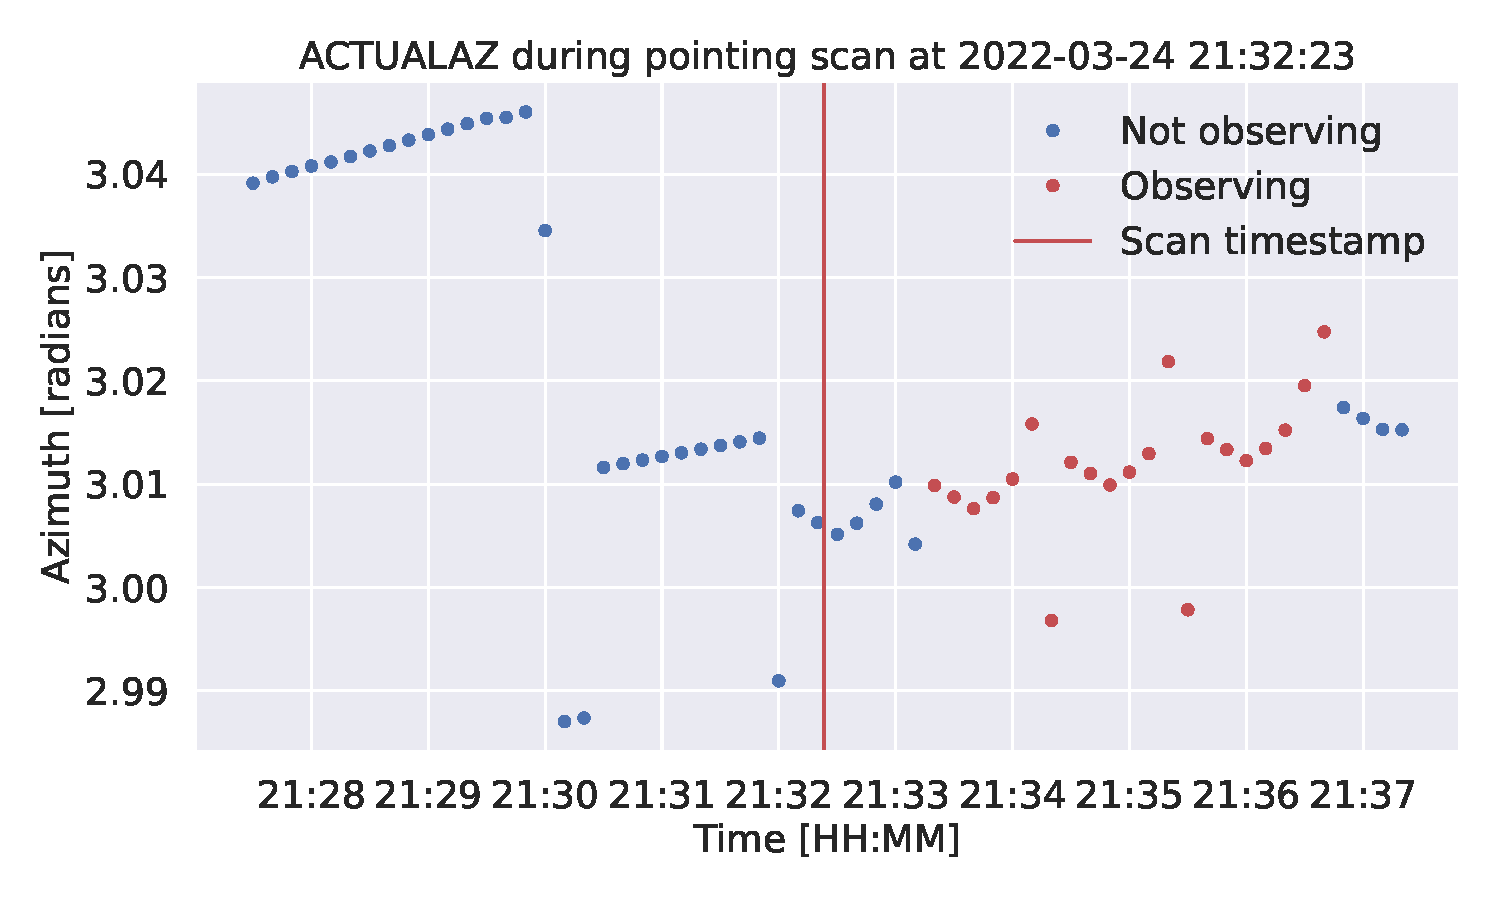
\includegraphics[width=\textwidth]{Feature during scans/scan_ACTUALAZ_335.pdf}
        \caption{Azimuth angle}
        \label{subfig:scan_az}
    \end{subfigure}
    \begin{subfigure}[t]{0.49\textwidth}
       \centering
       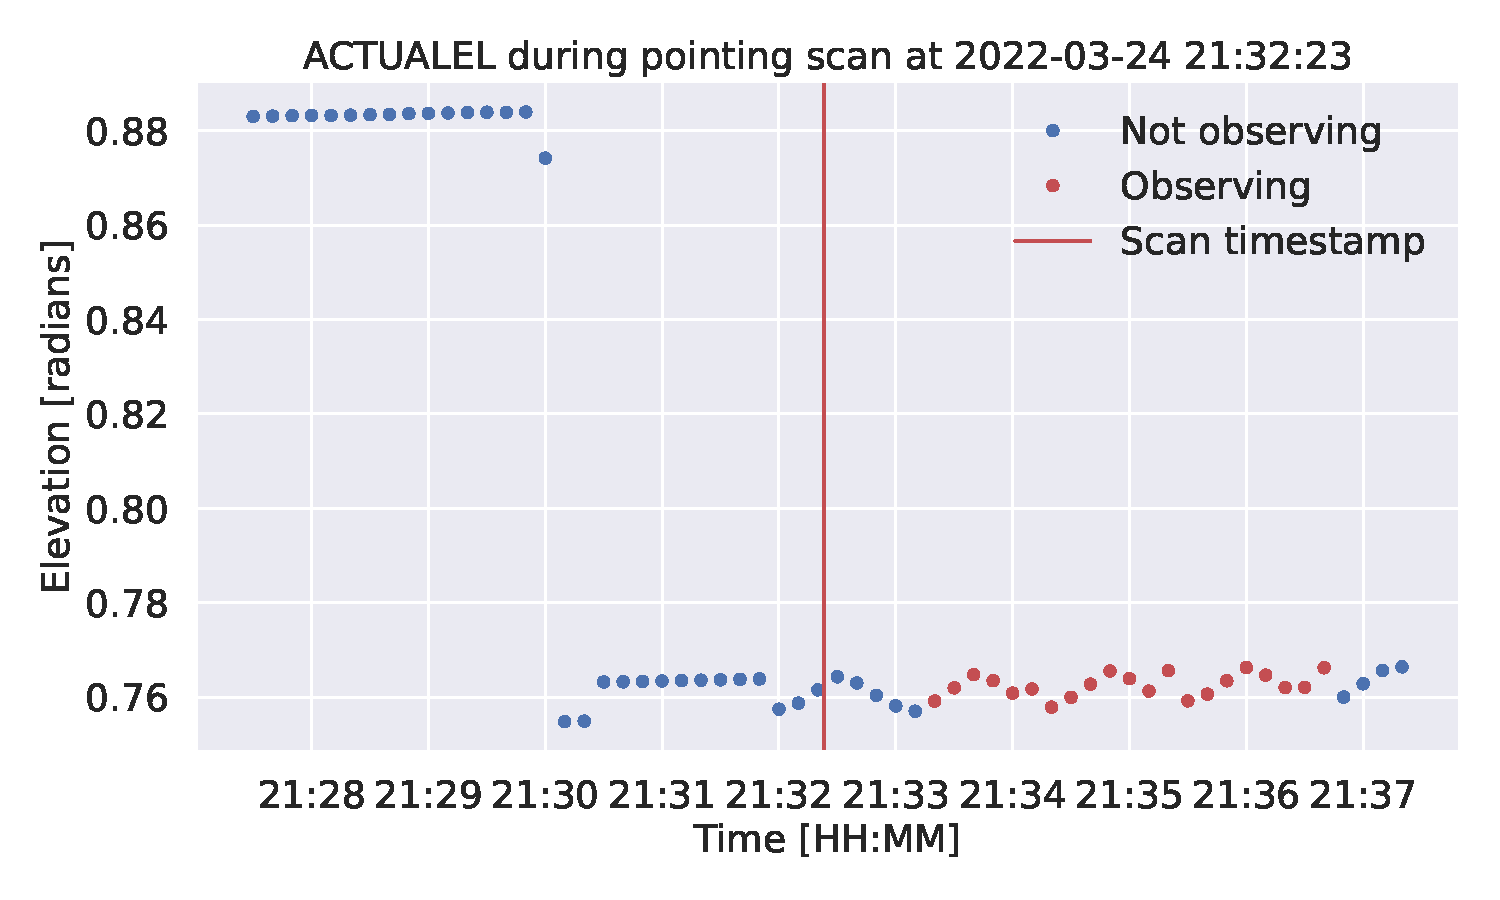
\includegraphics[width=1\textwidth]{Feature during scans/scan_ACTUALEL_335.pdf}
       \caption{Elevation angle.}
       \label{subfig:scan_el}
    \end{subfigure}
    \\~\\
    \begin{subfigure}[t]{0.49\textwidth}
        \centering
        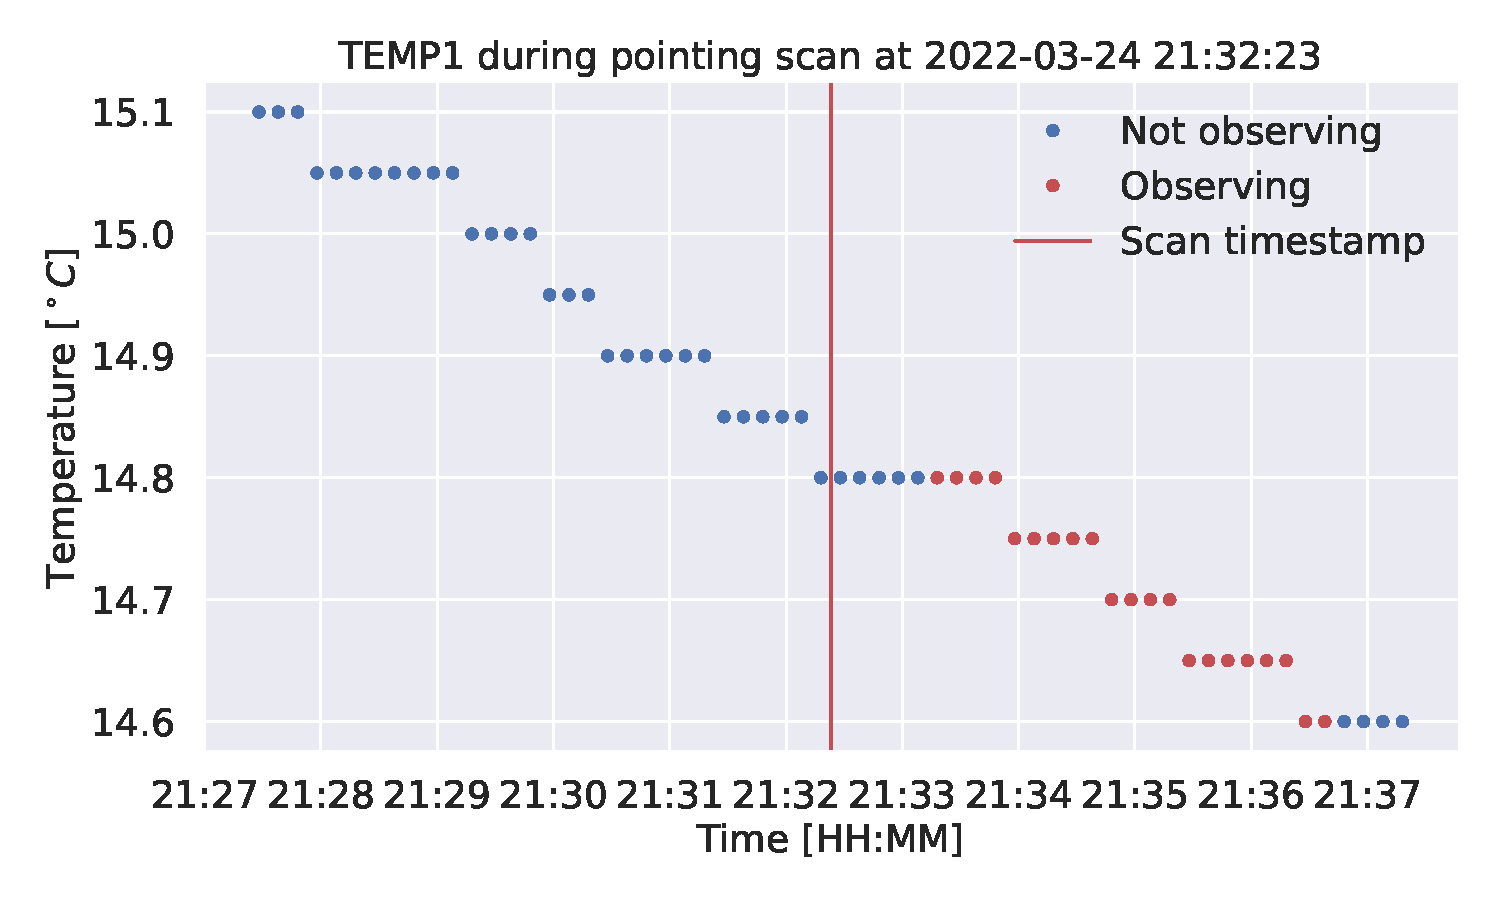
\includegraphics[width=\textwidth]{Feature during scans/scan_TEMP1_335.pdf}
        \caption{Temperature measurements at temperature sensor $1$.}
        \label{subfig:scan_temp1}
    \end{subfigure}
       \begin{subfigure}[t]{0.49\textwidth}
        \centering
        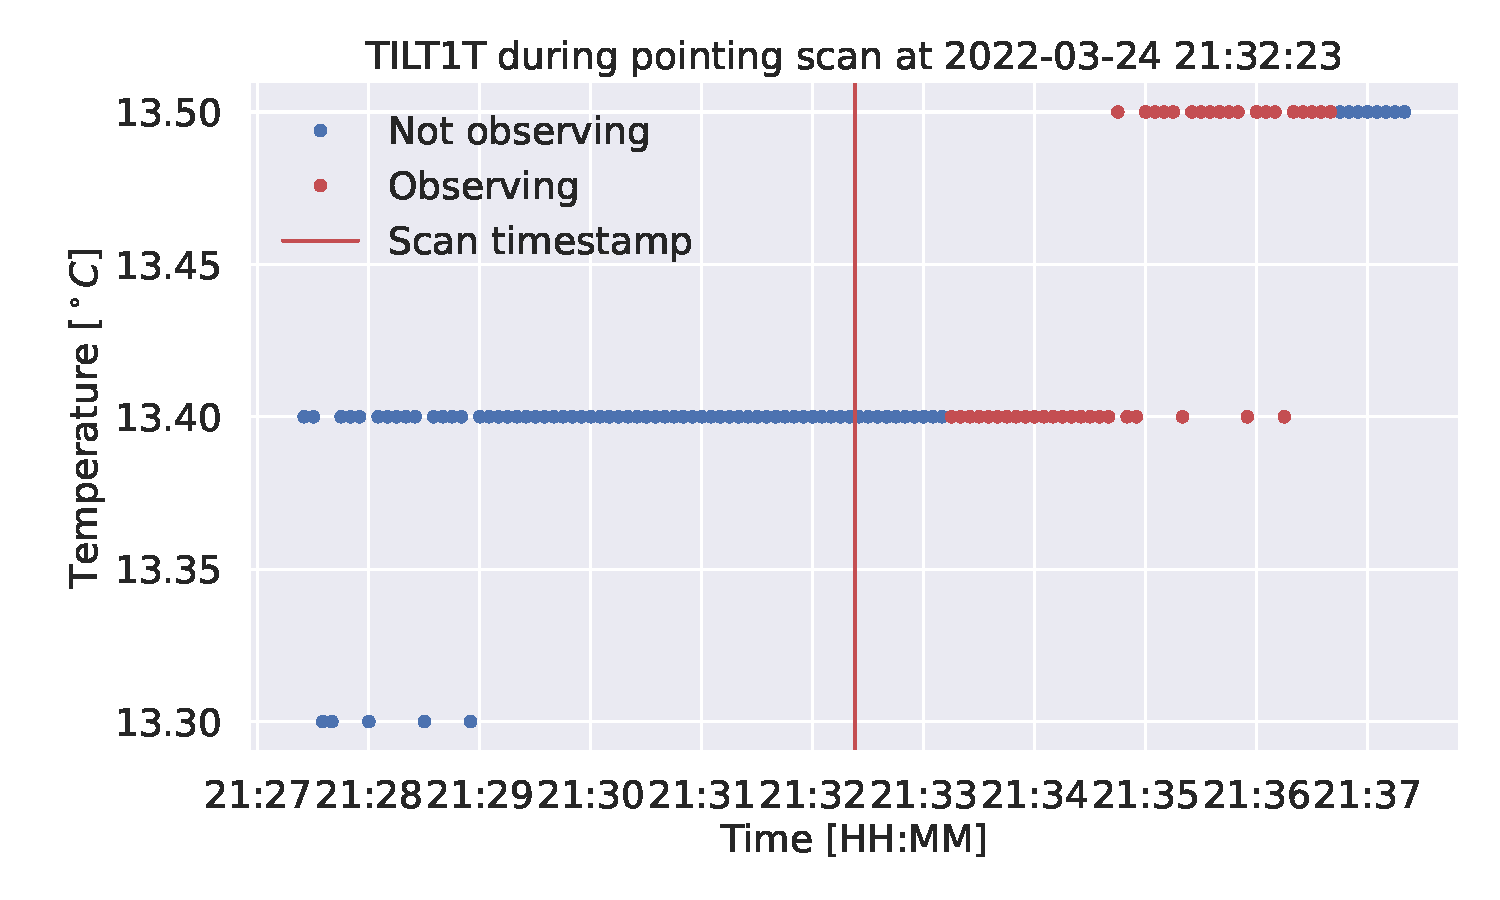
\includegraphics[width=\textwidth]{Feature during scans/scan_TILT1T_335.pdf}
        \caption{Temperature measurements at tiltmeter $1$.}
        \label{subfig:scan_tilt1t}
    \end{subfigure}
    \\~\\
    \begin{subfigure}[t]{0.49\textwidth}
        \centering
        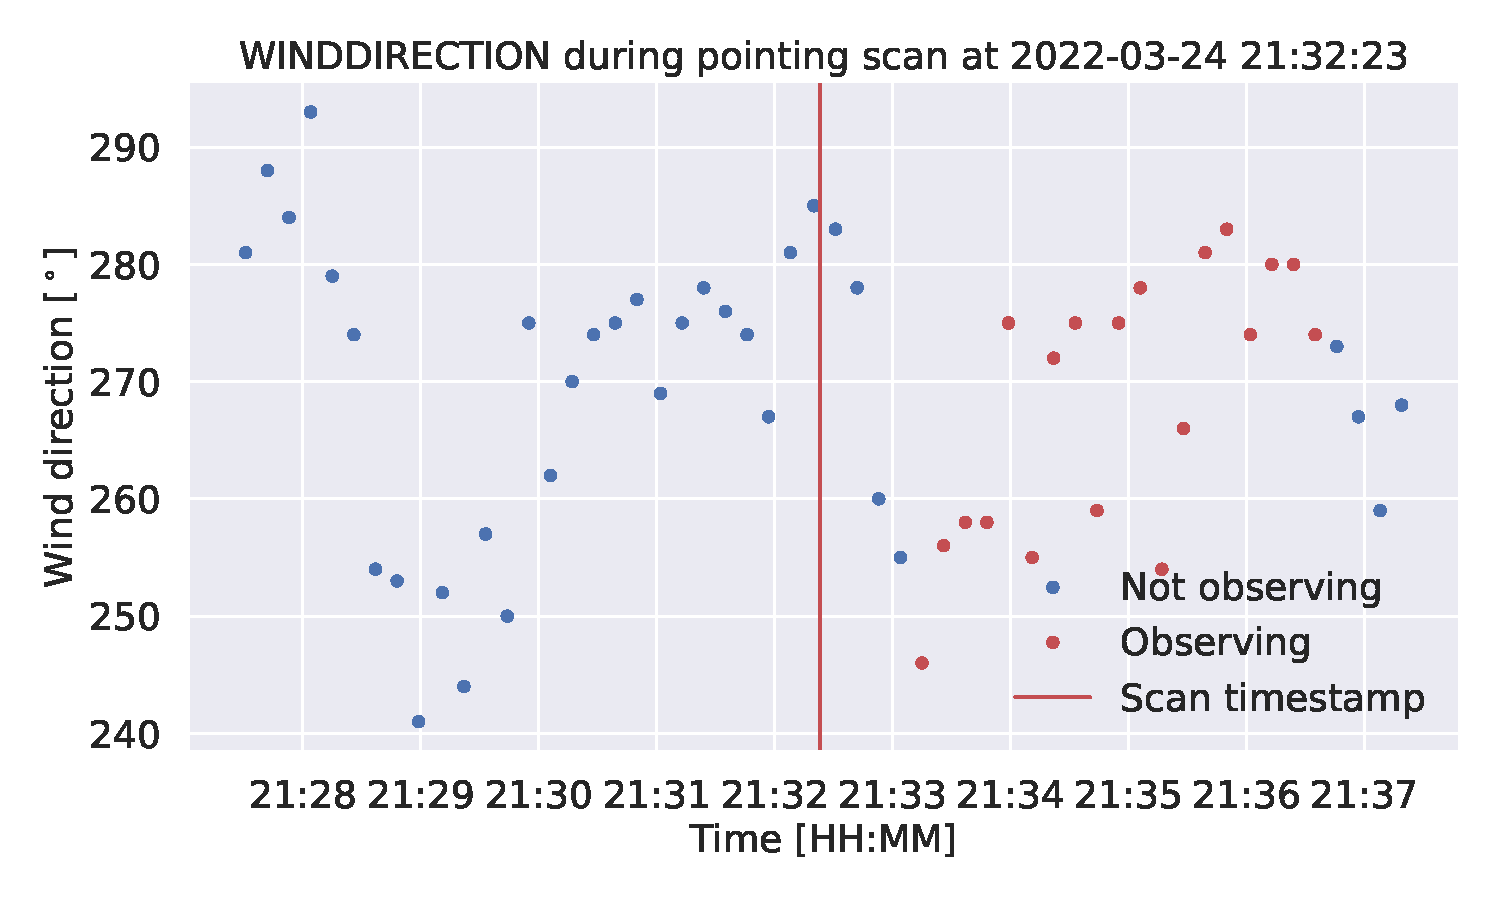
\includegraphics[width=\textwidth]{Feature during scans/scan_WINDDIRECTION_335.pdf}
        \caption{Wind direction data from the weather station, measured in degrees from North, where clockwise is positive angle direction.}
        \label{subfig:scan_winddir}
    \end{subfigure}
       \begin{subfigure}[t]{0.49\textwidth}
        \centering
        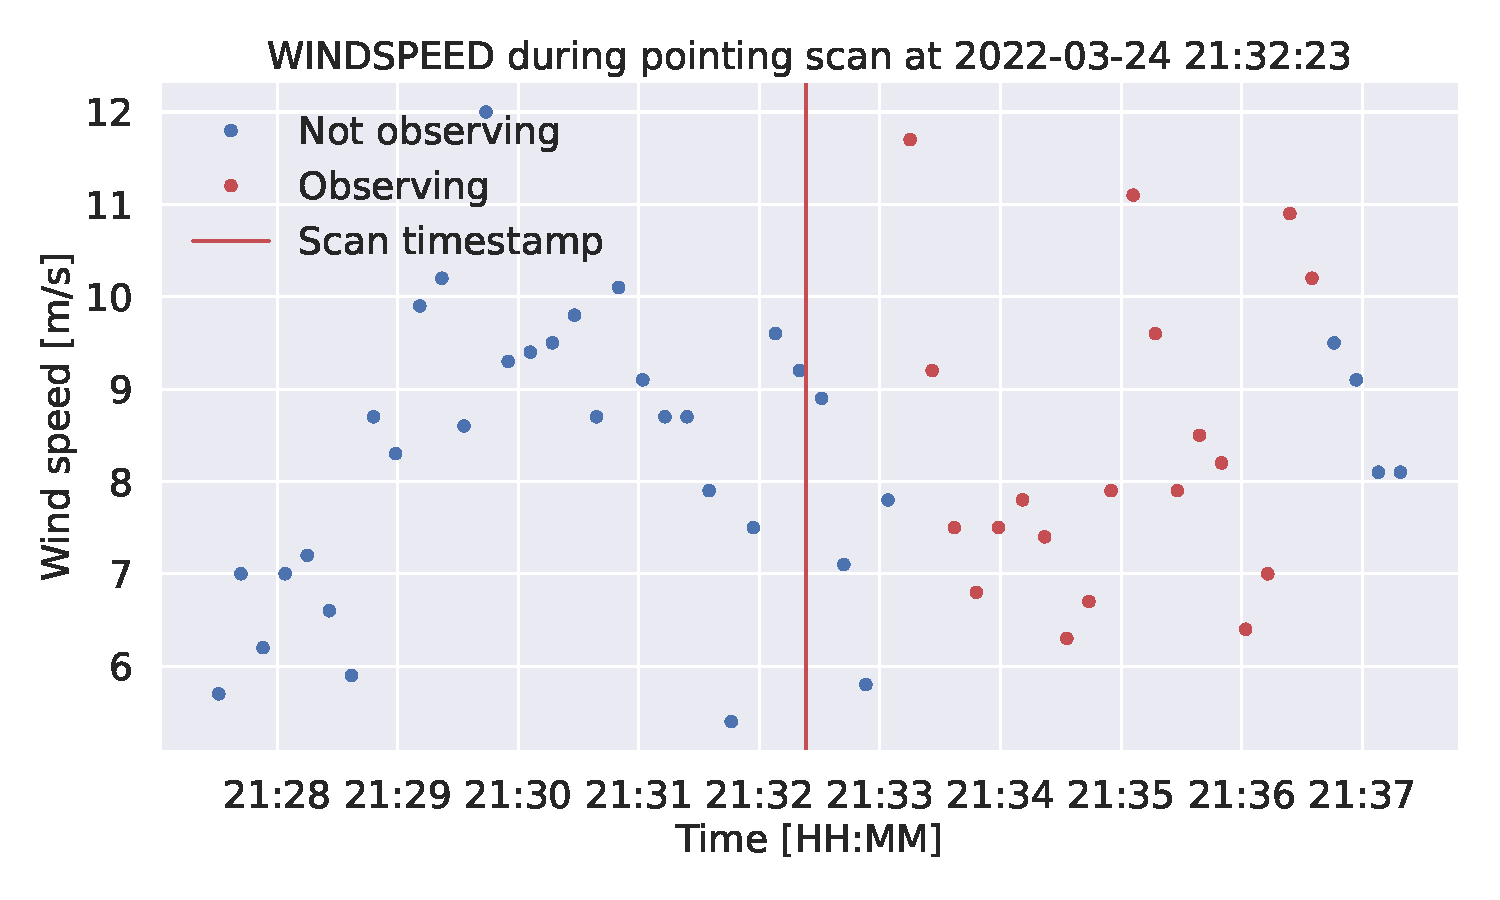
\includegraphics[width=\textwidth]{Feature during scans/scan_WINDSPEED_335.pdf}
        \caption{Wind speed data from the weather station.}
        \label{subfig:scan_windspeed}
    \end{subfigure}
     \caption{Timeseries plots of different sensory data before, during and a little after a pointing scan. The red line denotes the timestamp for a scan in the pointing scan database.
     The red dots are from when the telescope is observing, while the blue dots are when the telescope is idle or preparing to observe.}
     \label{fig:features_during_scans}
\end{figure}


\subsection{Pointing scan data}
A pointing scan is an observation of a source with known location, which is used to calibrate the pointing model.
There are two types of pointing scans: Line pointings and continuum scans.
Figure \ref{fig:features_during_scans} shows the information in the monitor database form a pointing scan.
\paragraph{Line pointing}
A line pointing involves pointing at an extended source. 
The telescope then makes ten scans, recording the flux intensity from the source, five vertically and five horizontally, around the center of the pointing, as shown in figure \ref{fig:line_pointings}.
The upper panel shows a high quality pointing scan and the lower panel shows a noise low quality pointing scan.
The cross-plot on the right side shows the line spectrum for each of the observations (center plus eight offset observations).

The flux from the source is integrated, and the resulting values are plotted as blue dots on the left-hand side of the plots.
A Gaussian is then fitted to these points, and the resulting amplitude, full width at half maximum (FWHM), and offsets are given in the table.

\begin{figure}[H]
    \centering
     \begin{subfigure}[b]{0.75\textwidth}
         \centering
         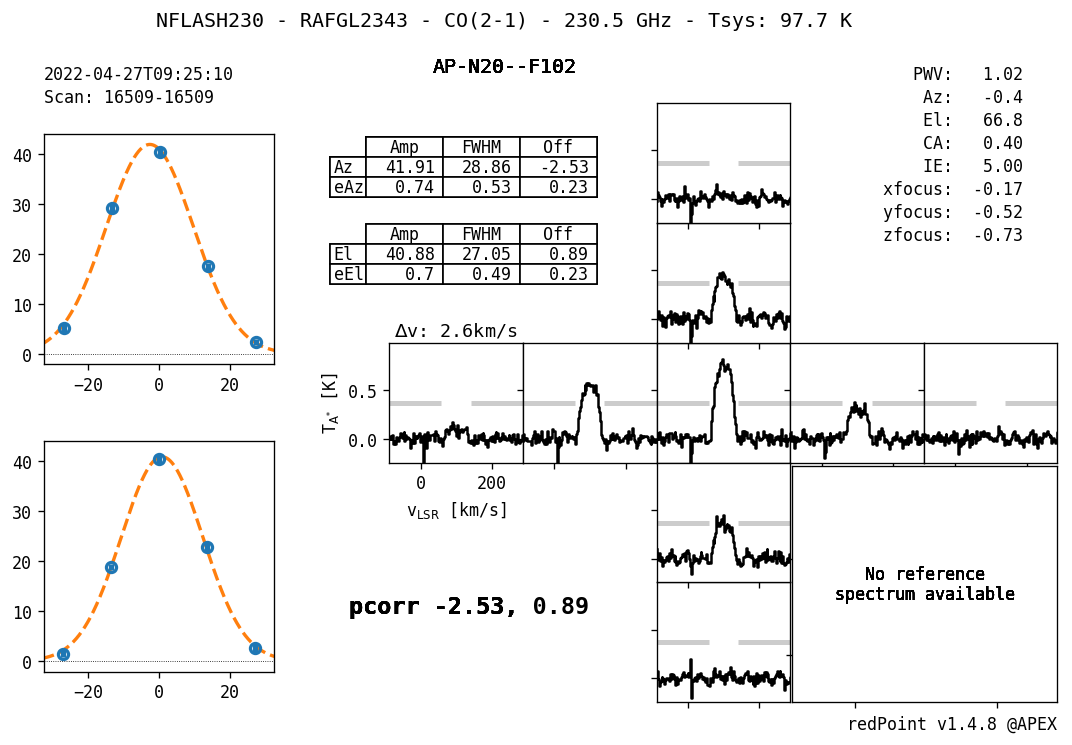
\includegraphics[width=\textwidth]{Pointing Scans/good_line.png}
         \caption{Line pointing with little noise and a good Gaussian fit.}
         \label{subfig:good_line}
     \end{subfigure}
    \\
     \begin{subfigure}[b]{0.75\textwidth}
         \centering
         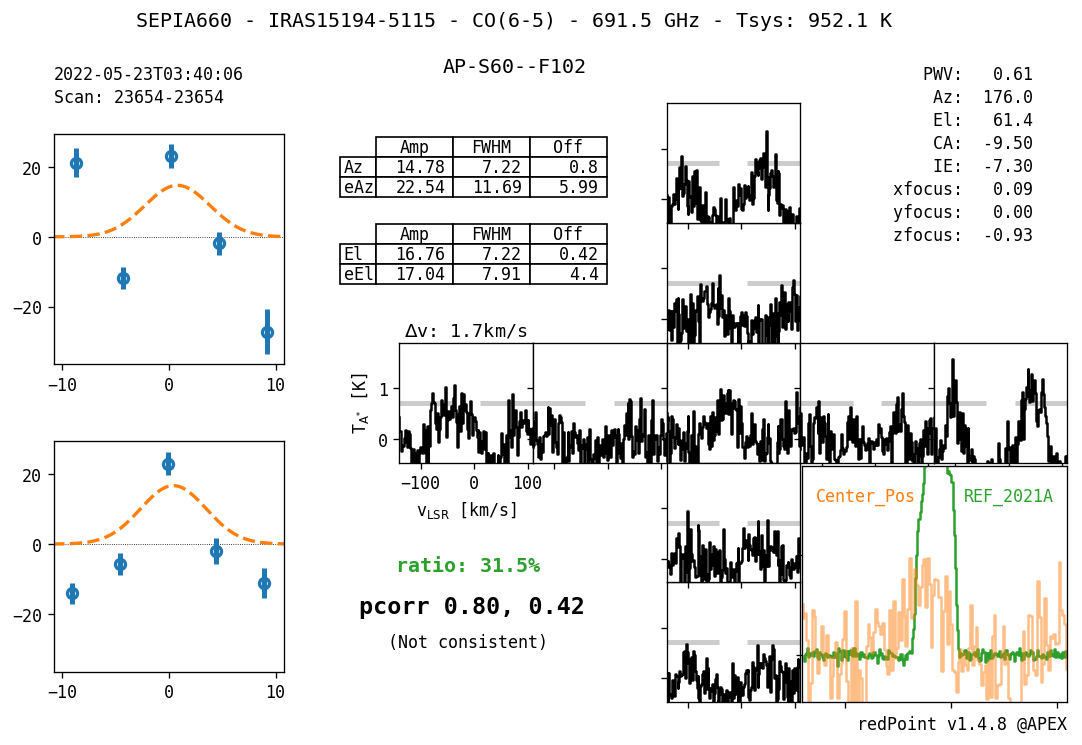
\includegraphics[width=\textwidth]{Pointing Scans/bad_line.png}
         \caption{Noisy line pointing with bad Gaussian fit.}
         \label{subfig:bad_line}
     \end{subfigure}
    \caption{The two figures show line pointing scans. a) is good and clean, and b) is noisy and unreliable. A Gaussian is fit both for the azimuth and elevation pointing.
    The amplitude, full width at half maximum, offset, and the uncertainty of these measures are shown for both fits.
    The figures also show the correction that was used during the pointing ($ca$ and $ie$), along with other metrics.}
    \label{fig:line_pointings}
\end{figure}

\paragraph{Continuum Scan}
Not all sources have emission lines, and for these sources a contunuum scan is carried out instead. In this case, a source is continuously scanned in azimuth and elevation while recording the flux intensity.
A Gaussian curve is fitted to the recorded flux intensity to determine the offsets, amplitude, and full width at half maximum (FWHM).
Figure \ref{fig:continueous_pointings} show examples of continuum scans and the corresponding Gaussian fits.

\begin{figure}[H]
    \centering
     \begin{subfigure}[b]{0.75\textwidth}
         \centering
         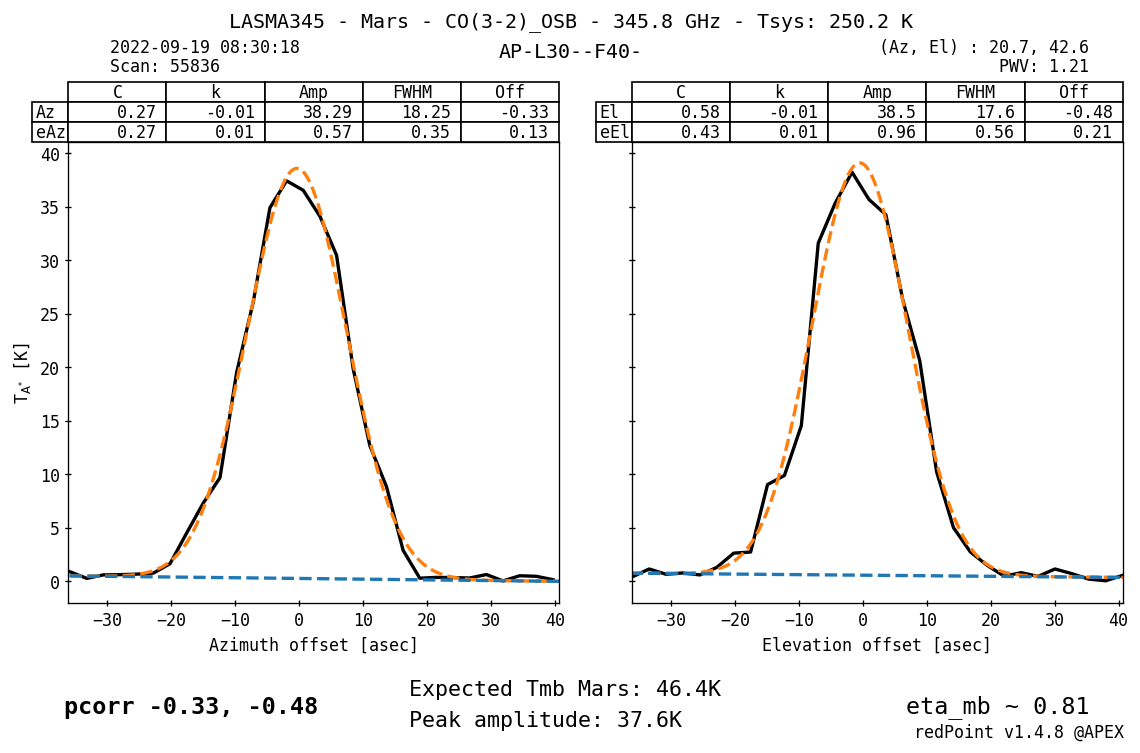
\includegraphics[width=\textwidth]{Pointing Scans/good_continuous.png}
         \caption{Line pointing with little noise and a good Gaussian fit.}
         \label{subfig:good_continuous}
     \end{subfigure}
    \\
     \begin{subfigure}[b]{0.75\textwidth}
         \centering
         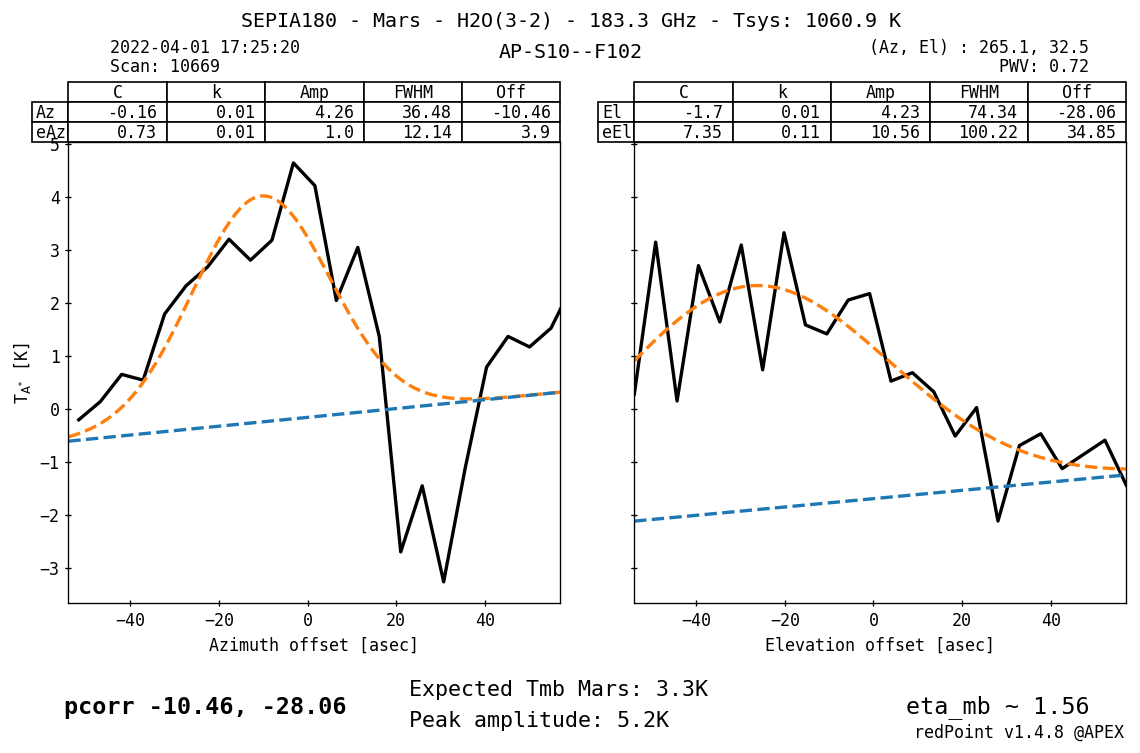
\includegraphics[width=\textwidth]{Pointing Scans/bad_continuous.png}
         \caption{Noisy line pointing with bad Gaussian fit.}
         \label{subfig:bad_continuous}
     \end{subfigure}
    \caption{The two panels show continuum pointing scans. a) is good and clean, and b) is noise and unreliable. A Gaussian is fit both for the azimuth and elevation pointing. The amplitude, full width at half maximum, offset, and the uncertainty of these measures are shown for both of the fits.}
    \label{fig:continueous_pointings}
\end{figure}



\paragraph{Pointing scan timestamp} 
In the main database, each pointing scan has a timestamp on the format YYYY-MM-DD HH:MM:SS, with second resolution. This timestamp does not reflect the the actual start of a pointing scan. Also, there is not information in the database itself that indicates whether the telescope is observing, but this information can be extracted from some dump files from the tiltmeter, which includes a flag indicating whether the telescope is idle, preparing to observe, or observing. Combining this flag with the timestamps, we can obtain the accurate start and end time of a pointing scan. However, these tiltmeter dump files are only available for some time periods.

\begin{itemize}
    \item Plots with scan times distribution
    \item proportion of scans we have the accurate time for
    \item What we did for hte other scans
    \item mention some deviation
\end{itemize}

\paragraph{Instruments}
The telescope is equipped with various observing instruments that operates at a variety of frequencies.
Table \ref{tab:instrument_usage} shows the frequency band each of the instruments cover,
along with the number of times they were used for a pointing scan throughout the year of $2022$.\\

The broad range of frequencies at which astronomical phenomena emit electromagnetic radiation requires observation across a wide range of frequencies to study these phenomena comprehensively.
A complete list of instruments and descriptions can be found at APEX's \href{https://www.eso.org/sci/facilities/apex/cfp/cfp110/instrument_summary.html.html}{website}.

\begin{table}[H]
    \centering
    \caption{The number of times each instrument was used for a pointing scan in $2022$. There are $8847$ scans in total.}
    \begin{tabular}{lcr}
        \toprule
        Instrument & Frequency band [GHz] &\# of scans \\
        \midrule
        NFLASH230 & $200$-$270$ &3197 \\
        LASMA345  & $268$-$375$ &1861 \\
        NFLASH460 & $385$-$500$ &1394 \\
        SEPIA660  & $578$-$738$ & 856 \\
        SEPIA345  & $272$-$376$ & 818 \\
        SEPIA180  & $159$-$211$ & 359 \\
        HOLO      & - & 225 \\
        ZEUS2     & - & 103 \\
        CHAMP690  & - &  34 \\
        \bottomrule
        \end{tabular}
        \label{tab:instrument_usage}
\end{table}



\subsection{Tiltmeter dump files}
The tiltmeter dump files is a small part of the database, and are only used to analyze when pointing scans start and end.
There are 280 of these files, and all have filenames on the format "Tiltmeter\_YYYY-MM-DD.dump", which indicates which date the data is from.
These files contrain 7 columns, which are datetime, azimuth, elevation, tilt1x, tilt1y, tilt1t and lastly the scan flag.
For our purpose, only the datetime and scan flag are interesting.
Table \ref{tab:tiltmeter_example} show an extract of the datetime and scan flag columns from one of the tiltmeter dumps.

\begin{table}[H]
    \centering
    \caption{Extract from a tiltmeter dump file.}
    \begin{tabular}{cc}
        \toprule
        Datetime & Scan flag \\
        \midrule
        2022-11-13T02:23:37 & IDLE \\
        2022-11-13T02:23:38 & IDLE \\
        2022-11-13T02:23:39 & PREPARING \\
        2022-11-13T02:23:40 & PREPARING \\
        $\vdots$ & $\vdots$ \\ 
        2022-11-13T02:23:52 & PREPARING \\
        2022-11-13T02:23:53 & PREPARING \\
        2022-11-13T02:23:55 & OBSERVING \\
        2022-11-13T02:23:56 & OBSERVING \\
        2022-11-13T02:23:57 & OBSERVING \\
        \bottomrule
    \end{tabular}
    \label{tab:tiltmeter_example}
\end{table}